\vspace{-0.5em}
\section{Methodology of GLARE}
\vspace{-0.5em}

\begin{figure}[t]
    \centering
    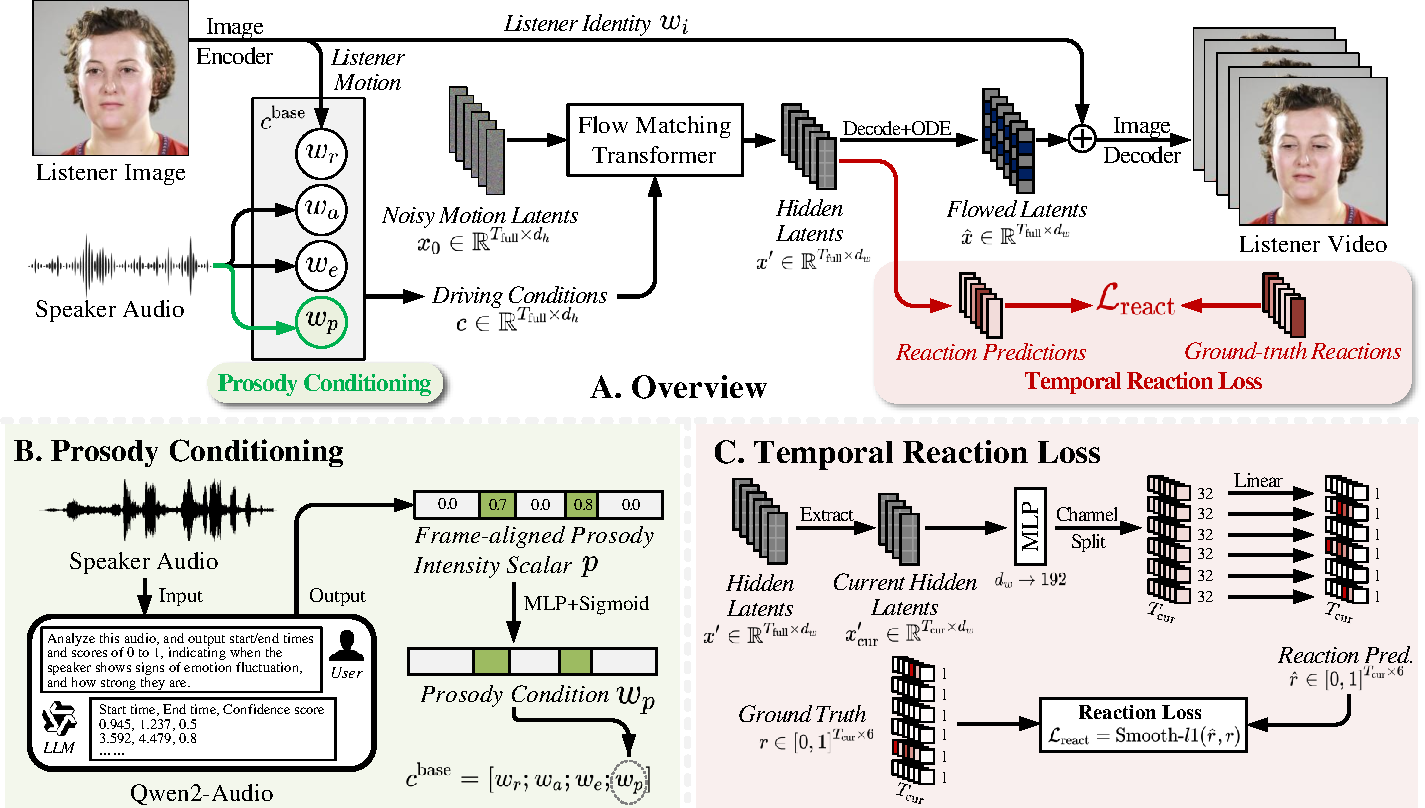
\includegraphics[width=\linewidth,keepaspectratio]{files/overview2.pdf}
    \vspace{-1.2em}
    \caption{Overview of our Prosody-conditioned Reacting Listener GLARE. Given speaker audio, a listener reference image, and temporal context, our model predicts listener motion latents using a conditional flow matching transformer (FMT). We further introduce prosody conditioning to capture speaker-side temporal prosodic variations, and a temporal reaction loss to explicitly supervise frame-wise listener reactions. The resulting motion latents are decoded into listener video frames.}
    \vspace{-1.2em}
    \label{fig:overview}
\end{figure}

\subsection{Preliminaries}

We present the overview of our listener GLARE in Fig. \ref{fig:overview}.A. Similar to FLOAT~\cite{ki2025float}, given a listener source image $S$ and a speaker audio segment $a$, the goal is to synthesize a listener motion-latent trajectory that can be decoded into listener video frames. We use LIA~\cite{wang2022lia} as a frozen image autoencoder to extract listener reference motion latent $w_r\in\mathbb{R}^{(T_{\text{prev}}+T_{\text{cur}})\times d_r}$\footnote{$d_r$, $d_a$, $d_e$, $d_{p}$, $d_w$ are channel dimension of $w_r$, $w_a$, $w_e$, $w_{p}$ and $x$. $d_h$ is the hidden dimension of FMT. \label{footnote1}} 
and identity latent $w_i$ from $S$, and use Wav2Vec2 \cite{baevski2020wav2vec} to encode $a$ into audio latents $w_a\in\mathbb{R}^{(T_{\text{prev}}+T_{\text{cur}})\times d_a}$\textsuperscript{\ref{footnote1}}. Note that we utilize $T_{\text{prev}}+T_{\text{cur}}$ frames of audio for generation, where $T_{\text{cur}}$ denotes current frames for listener motion generation, $T_{\text{prev}}$ indicate previous frames of audio context. Additionally, an emotion encoder \cite{pepino2021emotion} is used to encode the audio into an emotion latent $w_e\in\mathbb{R}^{(T_{\text{prev}}+T_{\text{cur}})\times d_e}$\textsuperscript{\ref{footnote1}} to represent speaker emotions. $w_r$, $w_a$, and $w_e$, along with $w_{p}$ (introduced in Sec \ref{sec:prosody_cond}), jointly construct the driving condition $c$. We then use $c$ is to modulate noisy latents $x=[x^{\text{ref}};x^{\text{prev}};x^{\text{cur}}]\in\mathbb{R}^{T_{\text{full}}\times d_w}$\textsuperscript{\ref{footnote1}} covering $T_{\text{full}}=T_{\text{ref}}+T_{\text{prev}}+T_{\text{cur}}$ frames, where $T_{\text{ref}}$ is reference listener frames providing more listener-side contexts. We adopt a DiT-style transformer \cite{peebles2023scalablediff} to predict the vector fields via flow matching \cite{lipman2022flow,ki2025float}. The vector fields will be further solved into listener flowed latent $\hat{x}$, which will be integrated with listener identity latent $w_i$ and decoded into video frames.

\vspace{-0.5em}
\subsection{Prosody Conditioning}  \label{sec:prosody_cond}
\vspace{-0.5em}

While conventional audio-driven listener generation mainly relies on low-level acoustic representations, listener reactions are often triggered by fine-grained speaker-side temporal cues, such as emphasis, affective fluctuation, and non-monotone prosodic changes. To make the driving condition more sensitive to such conversational cues, we introduce a prosody conditioning branch, where we further extract a frame-aligned prosodic intensity timeline using Qwen2-Audio-7B-Instruct \cite{Qwen2-Audio} in addition to $w_r$, $w_a$, and $w_e$. The full prompt template is given in Appendix \ref{app:prosody_extraction}.

Specifically, as shown in Fig. \ref{fig:overview}.B, we use the Audio LLM \cite{Qwen2-Audio} to analyze the audio prosody and obtain timestamps indicating prosodic fluctuations, which will be further processed into a frame-aligned prosody intensity scalar $p\in[0,1]^{(T_{\text{prev}}+T_{\text{cur}})\times 1}$ for each sample, where larger values indicate stronger prosodic or temporal affective variation in the speaker's speech. The scalar prosody signal is then projected to a compact latent representation $w_{p}\in\mathbb{R}^{(T_{\text{prev}}+T_{\text{cur}})\times d_{p}}$\textsuperscript{\ref{footnote1}} using a simple MLP and Sigmoid layer.
We then integrate $w_{p}$ into driving conditions by channel-wise concatenation $c^{\text{base}}=[w_{r};w_{a};w_{e};w_{p}]\in\mathbb{R}^{T_{\text{Full}}\times d_c}$, where $t$ denotes a specific frame, and $d_c=d_r+d_a+d_e+d_{p}$. The $c^{\text{base}}$ is then projected from $d_c$ to $d_h$\textsuperscript{\ref{footnote1}} as the final driving conditions $c$.
% is the base channel dimensionality of driving conditions.





\subsection{Temporal Reaction Loss}

A key limitation of purely reconstruction-based listener generation is that the model may produce visually plausible motions while failing to align with conversationally meaningful reactions. To explicitly encourage temporally accurate listener behaviors, we introduce a temporal reaction loss based on frame-wise reaction annotations.

We consider six listener reaction categories according to our defintions in Sec. \ref{sec:reaction_taxonomy}. As shown in Fig. \ref{fig:overview}.C, let $x^{\prime}_{\text{cur}}\in\mathbb{R}^{T_{\text{cur}}\times d_w}$ denote the transformer hidden latents for current frames, we first map each hidden token to an intermediate representation $z=\mathrm{MLP}(x^{\prime}_{\text{cur}})\in\mathbb{R}^{T_{\text{cur}}\times192}$. We then factorize $z$ into six class-specific subspaces, each with 32 channels, where $z_t \rightarrow \{z_t^{(k)}\}_{k=1}^{6},\ z_t^{(k)}\in\mathbb{R}^{32},\ t=1,\dots,T_{\text{cur}}$. Each reaction subspace is reduced to a time-specific latent $\hat{r}\in[0,1]^{T_{\text{cur}}\times6}$ with a class-specific linear layer, followed by a sigmoid activation. With the annotated frame-wise reaction target $r\in[0,1]^{T_{\text{cur}}\times6}$, we apply Smooth-L1 supervision:

\vspace{-1em}
{
\footnotesize
\begin{equation}
    \mathcal{L}_{\text{react}}=
    \frac{1}{T_{\text{cur}}}
    \sum_{t=1}^{T_{\text{cur}}}
    \mathrm{SmoothL1}(\hat{r}_t,r_t).
\end{equation}
}
\vspace{-1em}

This loss encourages the hidden motion representation to preserve reaction-aware temporal structure, improving not only the visual fidelity of listener motion but also the timing and type consistency of generated reactions.

\subsection{Training Objective and Inference}

The overall training objective is
{
\small
\begin{equation}
    \mathcal{L}=
    \mathcal{L}_{\text{fm}}
    +\lambda_{\text{vel}}\mathcal{L}_{\text{vel}}
    +\lambda_{\text{react}}\mathcal{L}_{\text{react}}.
\end{equation}
}Here, $\mathcal{L}_{\text{fm}}$ is the flow-matching loss on the predicted vector field, $\mathcal{L}_{\text{vel}}$ is the temporal velocity consistency regularizer \cite{ki2025float}, and $\mathcal{L}_{\text{react}}$ is the proposed temporal reaction loss. At inference time, the model takes the listener reference image, previous listener motion context, and speaker audio as input. The FMT predicts conditional vector fields, which are integrated with an ODE solver to obtain current listener motion latents. These motion latents are then decoded into video frames. 
% The reaction head is only used as an auxiliary training signal and does not alter the inference pipeline.